
\documentclass[12pt]{article}

\addtolength{\textwidth}{.8in}
\addtolength{\hoffset}{-.4in}
\addtolength{\textheight}{1in}
\addtolength{\voffset}{-1in}

\usepackage{amsmath}
\usepackage{graphicx}
\usepackage{upquote} % to convert funny quotes to straight quotes
\usepackage{amsfonts}
\usepackage{multicol}
\usepackage{paralist}
\usepackage{icomma}  % no spaces after commas
\usepackage{hyperref}  % links
\setlength{\parindent}{15pt}

\renewcommand*{\thefootnote}{\fnsymbol{footnote}}


\begin{document}

\begin{center}
\begin{Large}
DATA 219 Notes -- Apr. 19, 2018
\end{Large}
\end{center}

\section{``Special'' data types}

There are a number of special types of data that require somewhat different 
techniques to analyze that what we've learned so far. One example is
\textit{time-series data}, where observations are made at regular, fixed
points in time and one might be interested in identifying overall trends
(``stays at our hotel are going up''), seasonal contributions within those
trends (``summers have more customers in general than winters do''), and noise
components that may obscure both effects (``we just had a bad year last
year.'') A whole body of literature has arisen to treat time series with
specialized techniques.

Another example is \textit{free-text data}, or \textit{natural language data},
where the ``data'' is comprised of actual written sentences in a language like
English. This very unstructured stream can be analyzed using a bevy of
specialized techniques, from simple word counts to sequences of words
(``\textit{n-grams}'') to full parsing of sentences, and uses things like
``stemming'' algorithms to recognize that ``jump'' and ``jumping'' represent the
same basic concept.

Yet another example is \textit{geographic data} used to represent points or
areas on Earth. Longitude and latitude, along with a set of transformational
functions, can be used to annotate data about events and perform computations
to learn from them. All of these topics deserve their own course, and can only
be hinted at here.

\section{Graph-based data}

One other special data type which we'll spend some time on in this lesson is
\textbf{graph-based} (or \textbf{network-based} data. It is rapidly becoming
one of the most important types of data in the world, especially in view of
the rise of our highly interconnected world (socially, culturally,
economically, \textit{etc.}) This type of data also a relatively ``new kid on
the block,'' which means that humankind is just now starting to get a handle on
how to analyze it. It's an exciting area to learn about because there's so
much (even relatively basic things) that's unknown and waiting to be
discovered.

The word ``\textbf{graph},'' as we'll use it here, has nothing to do with the
x-y plot that word typically invokes in one's mind. It is instead a special
kind of data structure, or paradigm for organizing data. Rather than rows in a
table, like we're used to, a graph, or \textbf{network}, consists of
\textbf{vertices} connected by \textbf{edges}. Here's an example:

\begin{center}
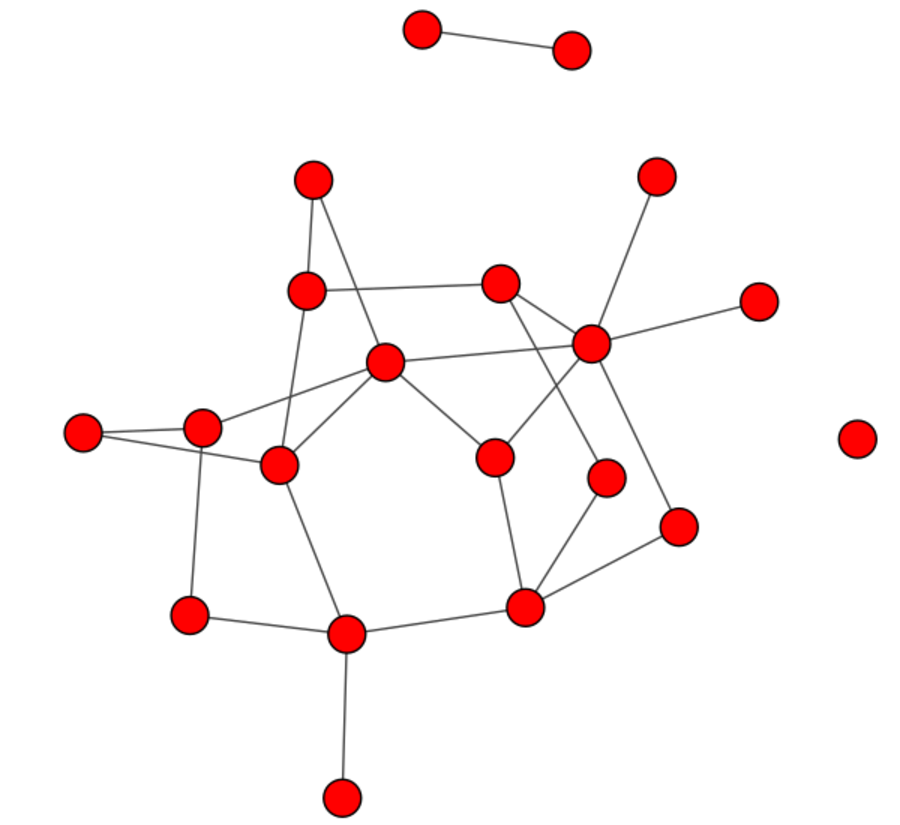
\includegraphics[width=0.7\textwidth]{first_example.pdf}
\end{center}

The circles are the vertices (also sometimes called \textbf{nodes}) and the
lines are the edges (sometimes called \textbf{links} or \textbf{arcs}). This
basic structure can be used to describe innumerable kinds of things:

\begin{compactitem}
\itemsep.1em
\item People and the social ties between them.
\item Computers on a network and the connections that join them.
\item International Banks and the transactions they have performed with one
another.
\item Physical locations and the routes/roads that connect them.
\item The pages on a particular website, and which ones link to which others.
\item Scholarly research papers and the citations they make of one another
\item \textit{Etc.}
\end{compactitem}

Part of what makes graph-based data so important and powerful is this plethora
of different applications. Aristotle, in fact, thought that this
vertex-and-edge thing was so universal that essentially all the information we
might want to conceive could be reduced to, and represent with, this
structure.

\subsection{Graph terms}

A whole specialized vocabulary has sprung up for talking about graphs and
their properties. Here are just a few common terms and their meanings:

\begin{itemize}
\itemsep.1em
\item \textbf{order} and \textbf{size} -- Colloquially, researchers sometimes
refer to the number of vertices in a graph as its \textbf{order}, and the
number of its edges as its \textbf{size}. (The ratio of these quantities
becomes a subject of interest as well.)
\item \textbf{to traverse} -- We use the verb ``\textbf{traverse}'' to mean
``follow a link from one node to another.'' This often comes up in the context
of searching for data in the graph, or finding a path through the graph with
certain features.
\item \textbf{directed/undirected} -- In the graph above, vertices are
connected by simple lines. This is called an \textbf{undirected} graph, and
means that there is no intrinsic directionality to the edges: a pair of
vertices simply either is, or is not, joined by an edge. Sometimes, we care
about which ``way'' the edge goes -- for instance, if we represented a family
tree, and the edges indicated parent/child relationships. Saying ``Sam is the
daughter of Betty Lou'' is very different than saying ``Betty Lou is the
daughter of Sam.'' For this kind of graph, we will add arrowheads to the edges
to show this. We typically say that one can only traverse directed links in
the forwards direction (\textit{i.e.}, in the direction of the arrow).
\item a \textbf{simple graph} vs. a \textbf{multigraph} -- With most graphs,
there is at most one edge between any two pairs of vertices. (Either the
locations have a road between them or not, either the two people are friends
or they're not, \textit{etc.}) In some cases, though, we may allow
\textit{multiple} edges per vertex pair. Perhaps in our application we need to
know how \textit{many} roads connect two locations, or how many communications
were sent from person A to person B. Graphs that allow this are called
\textbf{multigraphs}. Multigraphs are also typically allowed to have
\textbf{self-loops} (an edge from a vertex to itself) which is not allowed in
a simple graph.
\item \textbf{attributes} -- Both vertices and edges can be annotated with
special pieces of information called \textbf{attributes}. If vertices
represent people, perhaps we want to attach age or gender information to each
one. If edges represent communications between companies, maybe we want to
attach a date to each edge indicating when that communication took place. We
can depict attributes on the visual display (or not) through a variety of
means: text annotations, color/shape/size of the vertex, the thickness of the
line, \textit{etc.}
\item \textbf{weighted} graphs -- One particularly common type of \textbf{edge
attribute} is a number called the \textbf{weight} of the edge. This is often
depicted visually as the number positioned closely to the middle of the edge
itself. Typically this weight represents some sort of ``cost'' of ``using'' that
edge -- for instance, the distance (in feet) of the network cable between the
two computers, or the travel time (in minutes) of using the route from one
city to the other.
\end{itemize}
\begin{itemize}
\itemsep.1em
\item the \textbf{degree} (of a vertex) -- A vertex's ``\textbf{degree}'' is
simply the number of connections it has. In the diagram above, the bottom-most
node has degree 1, the one on the far right has degree 0, and the one at far
left has degree 2. For directed graphs, this notion expands to that of
``\textbf{in-degree}'' and ``\textbf{out-degree},'' which give the number of
incoming arrows and outgoing arrows, respectively.

\item the \textbf{degree sequence} (of a graph) -- If we take a census of the
degrees of all the vertices in a graph, and list them in descending order, we
get the \textbf{degree sequence} of the entire graph: The degree sequence of
the above graph, as you can tediously verify, is:

\begin{center}
6, 5, 4, 4, 4, 3, 3, 3, 3, 2, 2, 2, 2, 2, 1, 1, 1, 1, 1, 0
\end{center}

\item the \textbf{degree distribution} (of a graph) -- A graph's
``\textbf{degree distribution}''  can be thought of as a histogram of its
degree sequence: how many nodes are there of degree 0? Of degree 5? Of degree
10? \textit{Etc.} The degree distro can tell us a lot about the overall
properties and structure of a large graph. Here's the one for our example:

\begin{center}
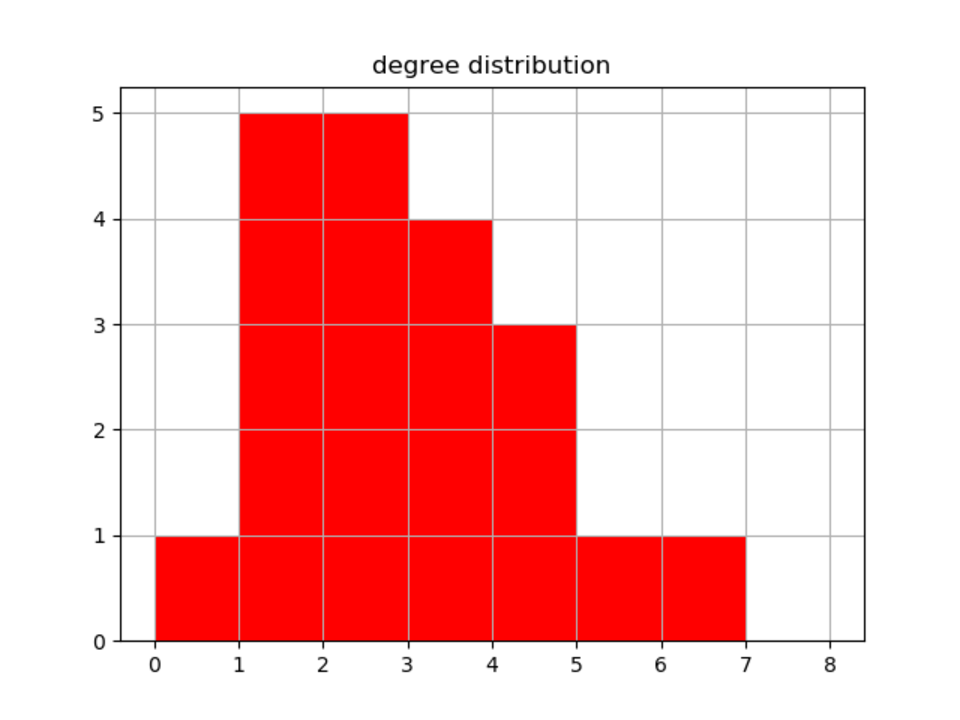
\includegraphics[width=0.7\textwidth]{degreeDistro.pdf}
\end{center}

\item \textbf{dyads}, \textbf{triads}, and \textbf{cliques} -- The word
\textbf{dyad} is essentially just a synonym for \textbf{edge}. It means, ``any
pair of nodes that are completely connected together,'' where ``completely
connected'' means ``have an edge between them.'' This term may seem unnecessary
until you consider the related terms \textbf{tryad} and \textbf{clique}. A
triad is a set of \textit{three} nodes which are \textit{completely} connected
to each other -- meaning, there is an edge between each pair of them. (Another
way to think of a triad is as a triangle $\triangle$.) ``Clique'' is the more
general word for ``some number of nodes, \textit{all of which} have an edge to
each of the others.'' We'll sometimes preface the word clique with a number,
and say ``this graph has a 5-clique'' or ``these eighteen vertices form an
18-clique.'' Note that a clique is a \textit{very} strong binding between the
vertices in a group -- they're totally inbred. Our example above, despite
having a fair number of edges, has only a single triad (can you find it?) and
no cliques of higher order.

\item a \textbf{complete} graph -- a (or ``the'') complete graph of a certain
order is simply one that has every possible edge. A complete graph of order 4
will be of size 6, since there are 6 possible different pairs of vertices, and
hence 6 possible edges.

\item \textbf{subgraph} -- a subgraph of a graph is simply one that has a
subset of its vertices and a subset of its edges. (Recall that ``subset'' does
not mean ``proper subset''; \textit{i.e.}, a set \textit{is} a subset of
itself.) Note: a clique, then, is a \textit{complete subgraph} of a certain
order. Sometimes we refer to an \textbf{induced subgraph} of a graph: this is
where we take (1) some subset of the original graph's vertices as the vertices
of the induced subgraph, and then (2) all the edges in the original graph that
connected vertices that we kept. In this way, specifying only the vertex
subset completely defines what the induced subgraph will be.

\item \textbf{connected} -- a graph is \textbf{connected} (sometimes called
``\textbf{fully connected},'' which means the same thing) if every vertex is
``reachable'' from every other vertex by traversing its edges. Our example
graph is not connected, because there's a pair of vertices at the top of the
page that don't connect to anything else (and also one lonely guy at the far
right).

Now what does ``connected'' mean for a directed graph? There are two notions:
``\textbf{strongly connected}'' and ``\textbf{weakly connected}.'' A directed
graph is strongly connected only if you can reach every vertex from every
other vertex only be traversing edges in the directions indicated. (No going
backwards on a one-way street.) It's weakly connected, on the other hand,
merely if it's connected once we \textit{ignore} the directionality of the
arrows.

\item \textbf{component} -- a \textbf{component} (also sometimes confusingly
called a ``\textbf{cluster}'') of a graph is a connected subgraph. Very simple.
Every graph will contain one or more components, each of which is a sort of
island which can't be reached from the others. Our example graph above has
three components. A common term is ``\textbf{giant component}'' which is used
to describe situations in which a graph is not fully connected...but almost
is. The big mass of nodes which are all connected to each other is called the
giant component to distinguish it from the onsie-twosie others that aren't
connected. Our example graph is of just this type.

\item \textbf{community} -- in contrast to components, a \textbf{community} is
a much vaguer, more nuanced concept. Component-ness has razor sharp criteria:
it's a component if all its nodes are reachable from each other and no other
nodes are, period. But a \textit{community} is an attempt to define a group of
nodes that are ``reasonably'' connected to each other, at least when compared
to their connections with those outside the community.

Imagine a small social network for a high school class in which most girls
were friends with most of the other girls, most boys were friends with most of
the other boys, but there was also the occasional boy-girl friendship. We
could identify the set of girl nodes, and the set of boy nodes, as
``communities'' because they are relatively cohesive internally and relatively
decoupled from one another. Note that you can't ever really definitively
declare: ``such-and-such a set of nodes \textit{is} a community, whereas this
set definitely \textit{isn't}.'' It's more subtle than that. There's degrees of
``community-hood'' depending on how dense the connections are within and
outside the community.

The subfield of \textbf{community detection} is devoted to algorithms that
will identify such groups according to various criteria. It is a critical part
of social network analysis.

\item \textbf{cycle} -- in a graph, a \textbf{cycle} is a group of nodes that
are connected in a ring: you can start at one, traverse edges to the others,
and then return to where you started.

\end{itemize}

\subsection{Special kinds of graphs}

Certain patterns arise often enough to deserve their own names. Here are some
special kinds of graphs:
\begin{itemize}
\itemsep.1em
\item \textbf{tree} -- A tree is a directed, connected graph with no cycles.
(A family tree is a good example of this, and often in fact we use the terms
\textbf{parents} and \textbf{children} to refer to the nodes that point to a
particular vertex, and the nodes that vertex points to, respectively.) A tree
has the interesting property that exactly one of its nodes will have no
parents (we call it the ``\textbf{root}'' of the tree) and that there is
exactly one traversable path from the root to any other node in the graph.

\item \textbf{DAG} -- Certain kinds of directed graphs, even if they're not
trees, must inherently be cycle-free to even make sense. For instance, the
graph of CPSC course prerequisites at
\url{http://cs.umw.edu/~finlayson/wiki-files/courses.png} (see below) must be
cycle free because the edges indicate required prerequisites, and if there
were a cycle in there...no one could ever graduate. These kinds of graphs are
called \textbf{DAGs} (``directed, acyclic graphs'') and are often used for
managing workflows in projects.

\begin{center}
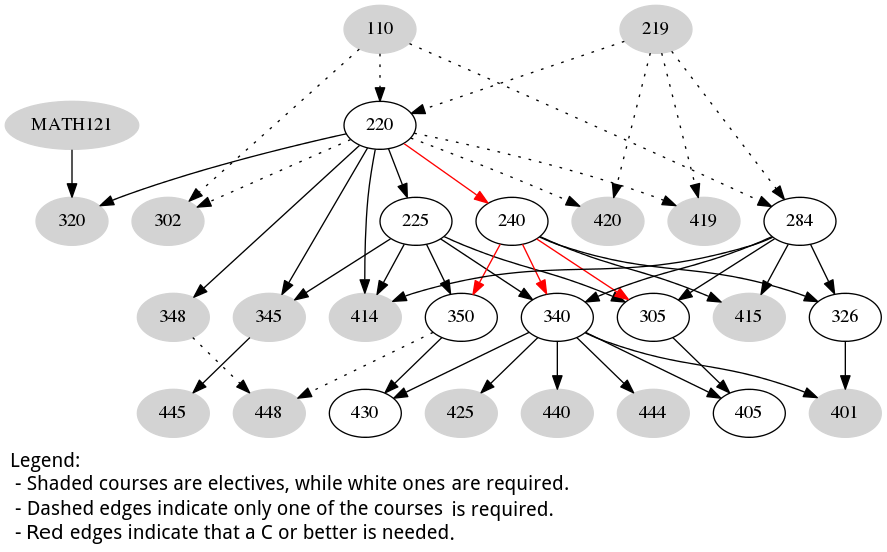
\includegraphics[width=0.9\textwidth]{courses.png}
\end{center}

\item \textbf{regular graph} -- A graph is \textbf{\textit{d}-regular} if all
of its nodes have degree $d$. The graph below, for instance, is 3-regular
(check it out!)

\begin{center}
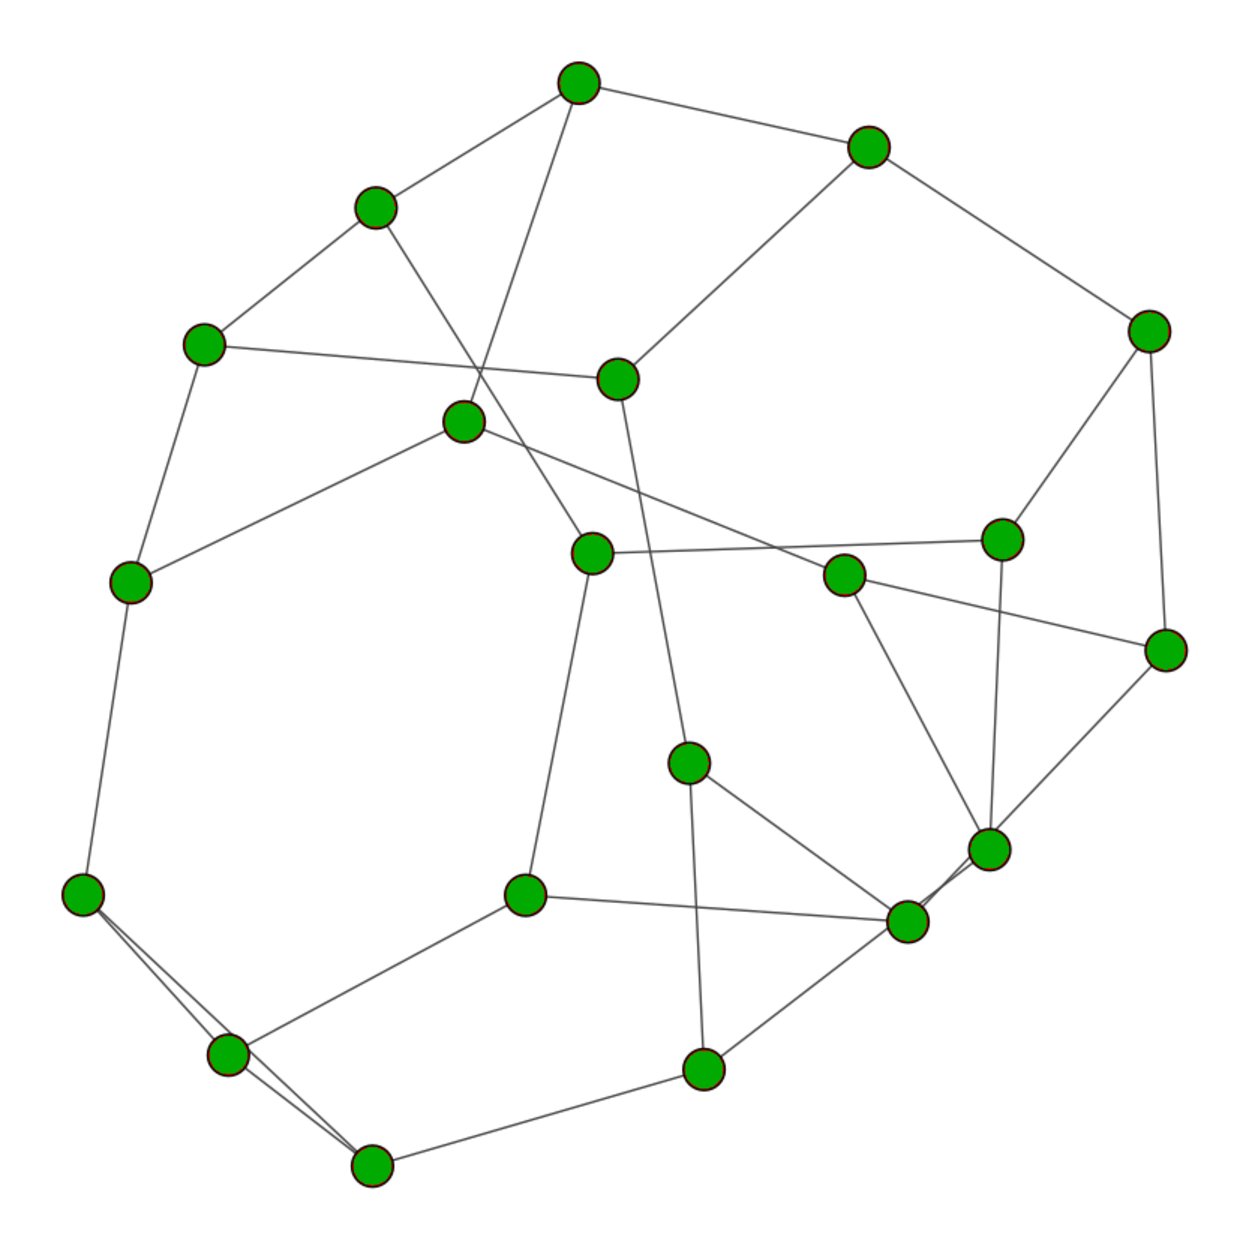
\includegraphics[width=0.6\textwidth]{regular.pdf}
\end{center}

\item \textbf{bipartite graph} -- A graph is \textbf{bipartite} if its
vertices can be split into two groups, and every edge \textit{only} joins a
vertex from one group with a vertex from the other. In a two-gender,
completely heterosexual society, the graph of dating relationships would be
bipartite. This kind of graph also comes up a lot in recommender systems: we
have two types of vertices: users, and (say) books. An edge between a user
and a book means that the user has purchased the book. (This is clearly
bipartite, because users never purchase each other, and neither do books.)

Bipartite graphs can be drawn with two rows of vertices, one of each type. All
the edges run across the middle.

\begin{center}
\includegraphics[width=0.4\textwidth]{bipartite.pdf}
\end{center}

\end{itemize}

\subsection{Representations}

When we're using a package like \texttt{igraph}, we often won't need to worry
too much about \textit{how} the graph we're working with is represented under
the hood. (Hint: it's not a bunch of circles and lines.) However, there will
be times when we need to retrieve, modify, or manipulate one or more of these
representations, so let's learn what they are.

\subsubsection{Edge list}

To a data scientist, perhaps the most straightforward way to represent a graph
is via an \textbf{edge list}, which is very much like a CSV file or DataFrame.
Each line gives two vertex names or IDs, which are connected by an edge.

\pagebreak
\begin{multicols}{2}
\begin{center}
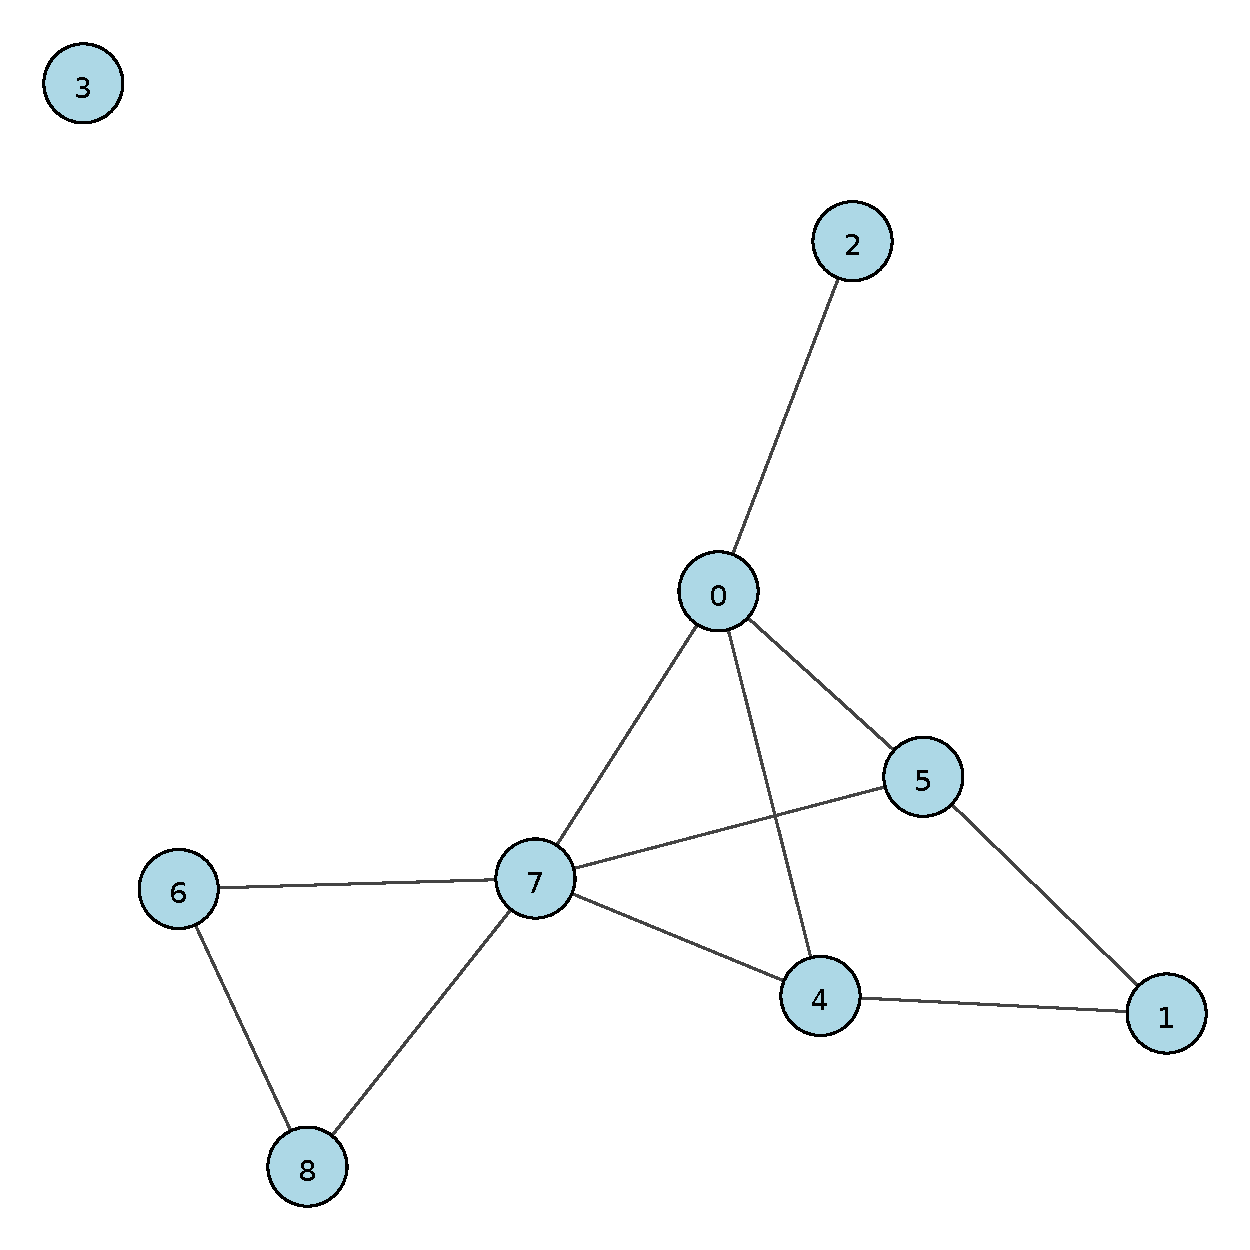
\includegraphics[width=0.48\textwidth]{second_example.pdf}
\end{center}
\columnbreak
  

Edge list:
\vspace{-.15in}
\begin{Verbatim}[fontsize=\small,samepage=true,frame=none]
      0,2
      0,4
      1,4
      0,5
      1,5
      0,7
      4,7
      5,7
      6,7
      6,8
      7,8
\end{Verbatim}
\end{multicols}

For a directed graph, the order of entries within a line would matter, of
course, but for an undirected graph, it doesn't.

\subsubsection{Adjacency matrix}

A graph's \textbf{adjacency matrix} is used in lots of different analysis
techniques. It's simply a matrix where every row (and column) corresponds to
one vertex. A ``1'' in an entry $(i,j)$ means ``yes, vertex $i$ and vertex $j$
are connected.'' Otherwise, they're not.

\begin{multicols}{2}
\begin{center}
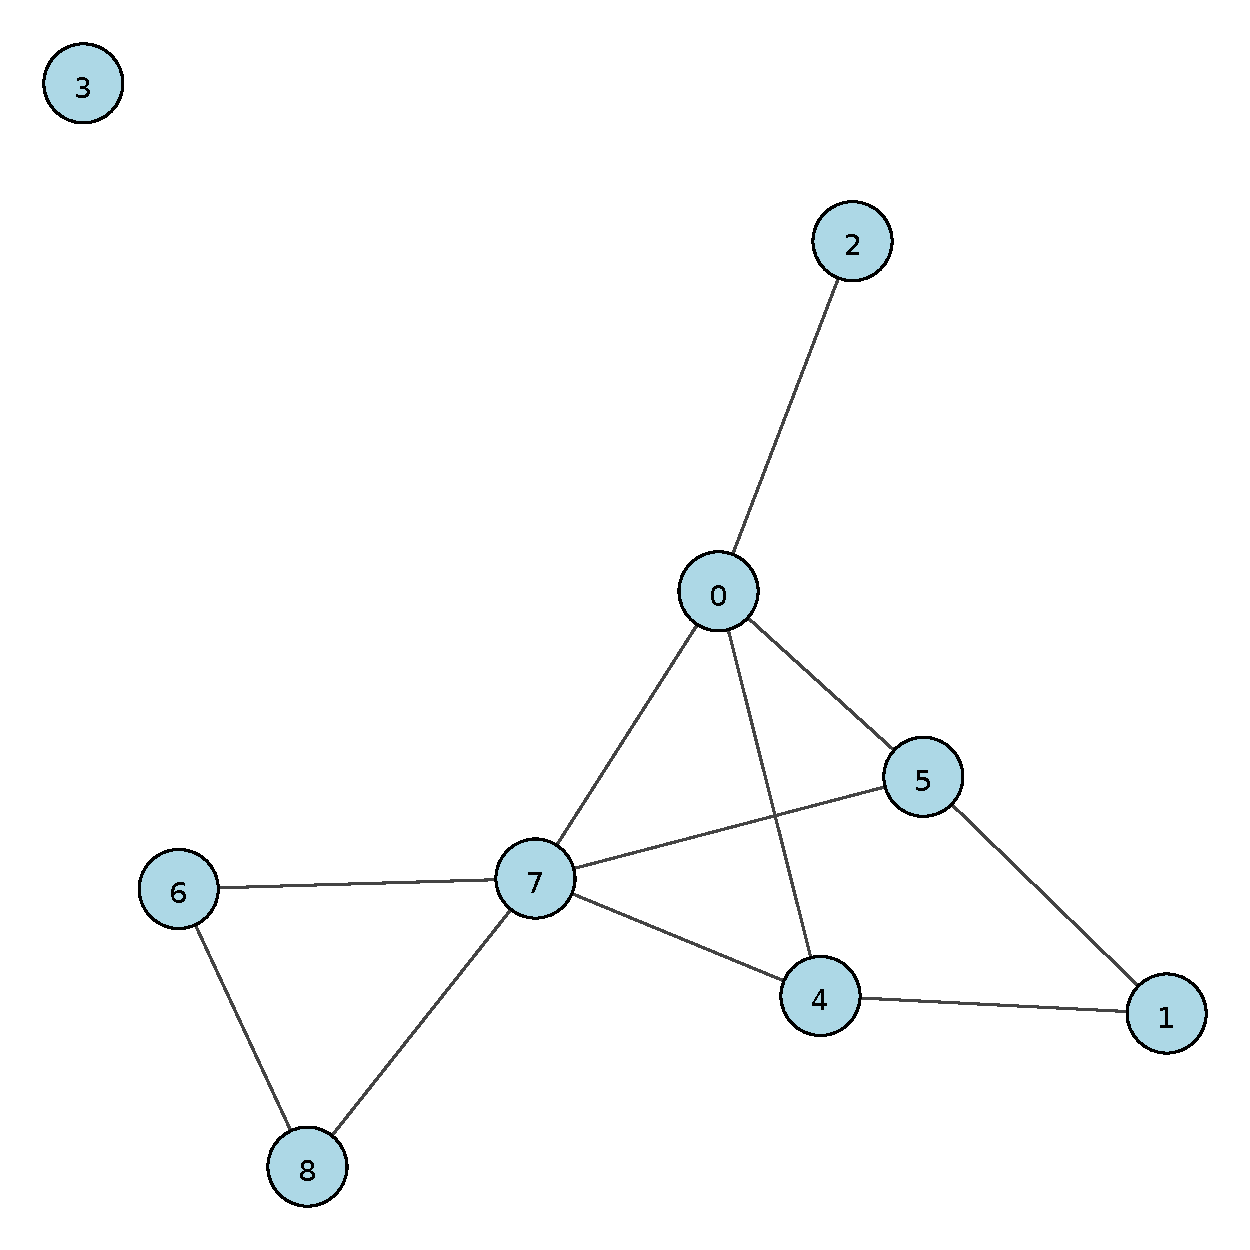
\includegraphics[width=0.48\textwidth]{second_example.pdf}
\end{center}
\columnbreak
Adjacency matrix:
\vspace{-.15in}
\begin{align*}
\begin{bmatrix}
  0 & 0 & 1 & 0 & 1 & 1 & 0 & 1 & 0 \\
  0 & 0 & 0 & 0 & 1 & 1 & 0 & 0 & 0 \\
  1 & 0 & 0 & 0 & 0 & 0 & 0 & 0 & 0 \\
  0 & 0 & 0 & 0 & 0 & 0 & 0 & 0 & 0 \\
  1 & 1 & 0 & 0 & 0 & 0 & 0 & 1 & 0 \\
  1 & 1 & 0 & 0 & 0 & 0 & 0 & 1 & 0 \\
  0 & 0 & 0 & 0 & 0 & 0 & 0 & 1 & 1 \\
  1 & 0 & 0 & 0 & 1 & 1 & 1 & 0 & 1 \\
  0 & 0 & 0 & 0 & 0 & 0 & 1 & 1 & 0 \\
\end{bmatrix}
\end{align*}
\end{multicols}

Note how for an undirected graph (as we have here) the adjacency matrix will
be \textbf{symmetric}, \textit{i.e.}, a mirror image across the main
(upper-left-to-lower-right) diagonal. Note also that for a high-order but
relatively low-size graph, the adjacency matrix will be \textit{huge} (and
``\textbf{sparse}'': mostly zeros), much larger than it needs to be.

\subsubsection{Adjacency list}

A much more compact version of the adjacency matrix (is the \textbf{adjacency
list}, which addresses the sparsity problem. Instead of a big $n\times n$
matrix with mostly zeroes, the adjacency list only gives us, for each vertex,
\textit{a list of the other vertices it connects to}. It looks like this:

\begin{multicols}{2}
\begin{center}
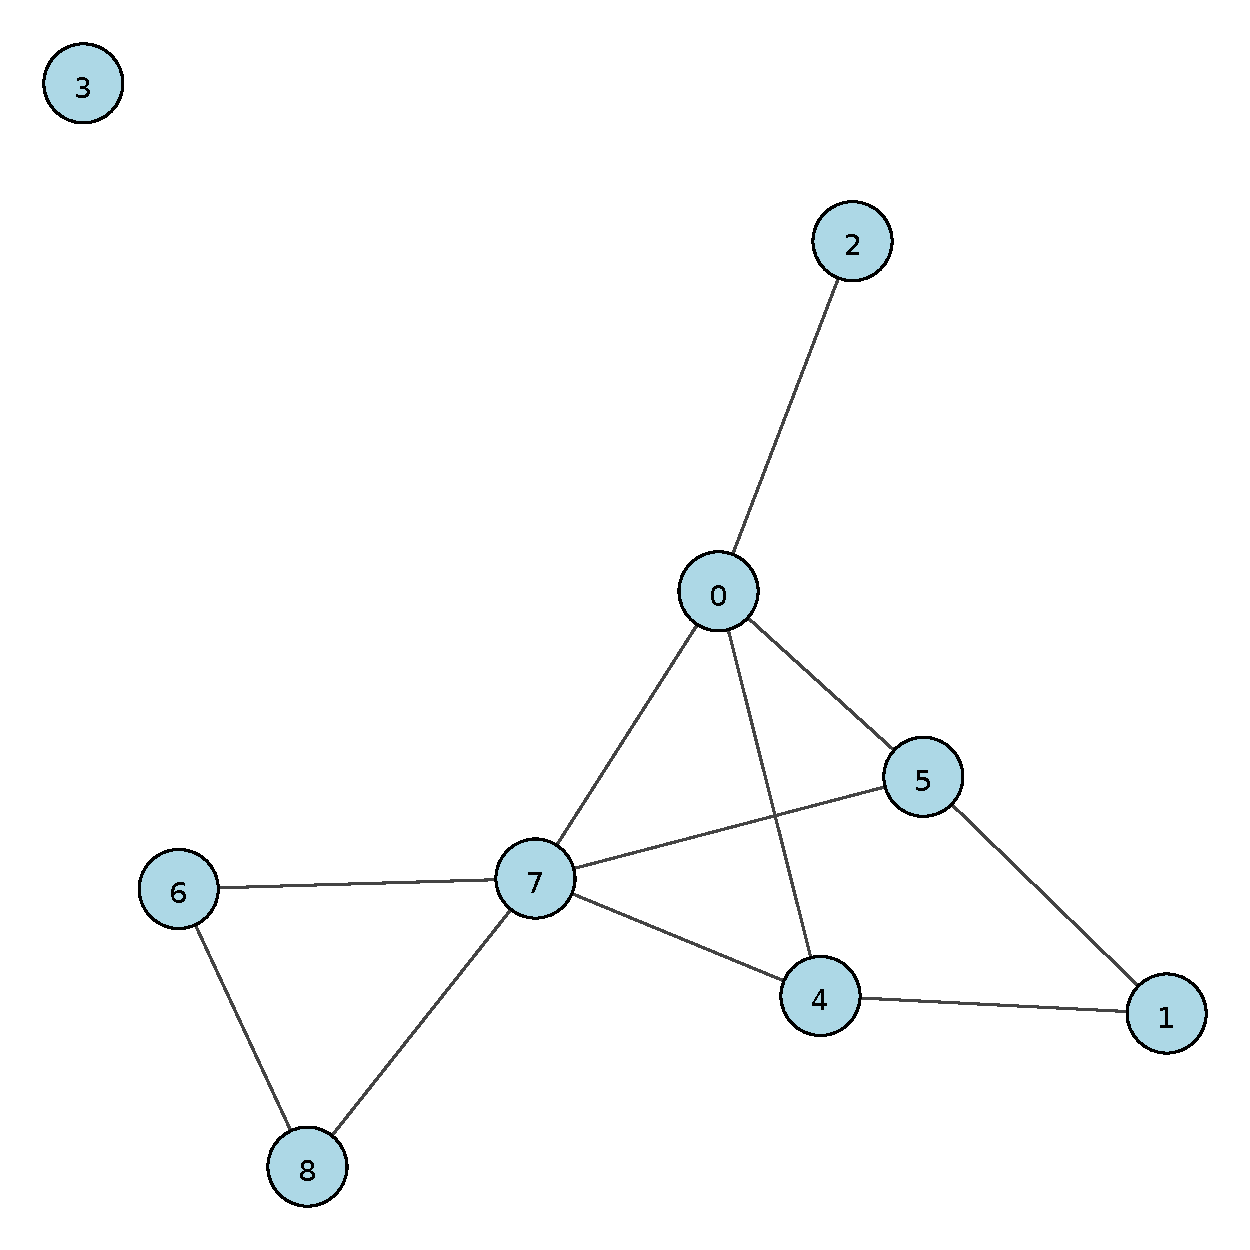
\includegraphics[width=0.48\textwidth]{second_example.pdf}
\end{center}
\columnbreak
Adjacency list:
\begin{Verbatim}[fontsize=\small,samepage=true,frame=none]
  0: [2, 4, 5, 7]
  1: [4, 5]
  2: [0]
  3: []
  4: [0, 1, 7]
  5: [0, 1, 7]
  6: [7, 8]
  7: [0, 4, 5, 6, 8]
  8: [6, 7]
\end{Verbatim}
\end{multicols}


\subsection{Descriptive measures}

Graphs are extremely expressive, but for that reason they're hard to get your
head around. If you look at a small graph (order 10, say), you can stare at it
long enough to figure out what the structure is: who's connected to whom,
where the cliques are, what the components are, \textit{etc.} But for anything
bigger, it's a maze. Looking at a two-dimensional representation doesn't
reveal much about the graph's inner properties. And it turns out that graphs
have many interesting inner properties that help explain its behavior in the
real world.

We've already seen one example of this, with the \textbf{degree distribution}.
This shows us, generally speaking, how many high-connected and low-connected
nodes we have, which may imply many things depending on the domain.

\subsubsection{Clustering coefficient}

Another variable of interest is the \textbf{clustering coefficient}, also
sometimes called the \textbf{transitivity}, of a graph. It measures how often
it's true that friends-of-a-friend are also friends. If we define a
``chevron''
($\wedge$) as two nodes sharing a neighbor (\textit{i.e.}, vertex A is
connected to B, and B is connected to C), the transitivity tells us what
fraction of the time this is a complete triangle ($\triangle$) (\textit{i.e.},
how likely it is that A is connected to C). This tells us something about how
tightly clustered the graph is: are people wrapped up in tight-nit balls, or
are their relationships more spread out throughout the society? (The
transitivity of the light-blue graph, above, is .36, whereas the original red
one was only .2.)

\subsubsection{Centrality measures}

A question that often arises in graphs is: which nodes are the most central?
By ``central'' we don't mean ``drawn near the center of the page,'' since that
is solely dependent on the layout algorithm, not the graph structure. What,
then, does ``central'' mean?

\vspace{.2in}
One measure is called \textbf{closeness centrality}. For a given node $x$,
suppose we calculate \textit{the sum of the length of the shortest paths
between $x$ and every other node.} This is called the ``\textbf{farness},'' and
will obviously be higher for nodes that are very far away from at least some
others. It will presumably be the lowest for nodes that are most centrally
located, since they are not hugely far from \textit{any} of the other nodes.

If we take the reciprocal of the farness, we get the ``\textbf{closeness},''
and often we normalize this by multiplying by the order of the graph (so we
can compare closeness values between graphs of different sizes.) The final
formula for the closeness centrality of a node $x$, then, is:
\begin{align*}
c_{\textrm{closeness}}(x) = \frac{N}{\sum_{v \in V} \textrm{dist(v,x)}}
\end{align*}

where $N$ is the order of the graph, $V$ are the vertices in the graph, and
``dist($a,b$)'' is the shortest distance\footnote{Also sometimes called the
``geodesic distance'' just to be confusing.} between two nodes $a$ and $b$.

By this measure, the most central vertex in the light-blue graph is 7 (with a 
$c_{\textrm{closeness}}$ of .444), followed by 0, 5, and 4. The ``least
close''
is node 3, with a measly .111.

\vspace{.2in}

A different way to think about centrality is in terms of information flow.
Suppose these vertices are actors in a social network. Which ones are most
crucial to a piece of news finding its way around to everyone? 

One way to measure this is with \textbf{betweenness centrality}. For a given
node $x$, we ask, ``of all the pairs of vertices $a$ and $b$, how often is $x$
on the \textit{shortest} path from $a$ to $b$?'' If information is to travel
from $a$ to $b$, it's probably most likely (though not certain) that it will
travel along the shortest path between those two nodes. So if $x$ is on a lot
of such paths, it means it will be a common conduit of information exchange
between others. We define this mathematically as follows:

\begin{align*}
c_{\textrm{betweenness}}(x) = \sum_{a,b \in V} \frac{\sigma(a,b|x)}{\sigma(a,b)}
\end{align*}

where the notation ``$\sigma(a,b)$'' means ``the number of shortest paths from
$a$ to $b$'' (there could be more than one of these, in case of a tie), and
where the notation ``$\sigma(a,b|x)$'' means ``the number of shortest paths
from $a$ to $b$ \textit{which pass through $x$}.''\footnote{Sometimes, we
normalize this by dividing by $(N-1)(N-2)$, to get it to be a number between 0
and 1 like the closeness centrality is.} The larger this number is, the
greater the chance that $x$ will participate in an exchange of information
between any two nodes.


Perhaps not surprisingly, for the light-blue case the same nodes are central
by both these measures. Node 7 has a (normalized; see footnote) betweenness
centrality of .184, followed by nodes 0, 5, and 4. One difference is between
nodes 1 and 8: $c_{\textrm{closeness}}(8)$ is higher than
$c_{\textrm{closeness}}(1)$ ($.348 > .333$), but $c_{\textrm{betweenness}}(1)$
is higher than $c_{\textrm{betweenness}}(8)$ ($.333 > 0$). This is because
although 8 is a bit closer to the heart of the action, he's not on
\textit{anyone's} shortest path to anyone else. (There's nobody better than
node 1, meanwhile, for getting info from 4 to 5.) Therefore, in terms of
information passing purposes, he's kind of useless.


\vspace{.2in}

Finally, for those who have linear algebra in their arsenal, there are various
ways of using \textbf{eigenvectors} of the adjacency matrix to measure
centrality. One of these algorithms is called \textbf{PageRank}, which you may
be familiar with since it made Google famous and the number one search engine
in the world. The idea is that the more central \textit{your neighbors} are,
the more central you're likely to be. (In terms of playground drama: a popular
person is not so much one with a lot of friends, but rather one with a lot of
\textit{popular} friends.)

The math involved is beyond the scope of this course, but if you've had some
matrix algebra it's not too hard, and of course \texttt{igraph} can do the
heavy lifting for us.


